% OLMo-only parallel-phase paper. This file deliberately does not edit the
% shared Phase 4 or Gemma manuscripts. All native evidence is development or
% methods tier and is named by append-only registry ID.
\documentclass[11pt]{article}

\usepackage[letterpaper,margin=0.72in,headheight=14pt]{geometry}
\usepackage[T1]{fontenc}
\usepackage[utf8]{inputenc}
\usepackage{lmodern}
\usepackage{microtype}
\usepackage{amsmath,amssymb}
\usepackage{booktabs,tabularx,array}
\usepackage{enumitem}
\usepackage{xcolor}
\usepackage{graphicx}
\usepackage{caption}
\usepackage{float}
\usepackage[most]{tcolorbox}
\usepackage{fancyhdr}
\usepackage{titlesec}
\usepackage{xurl}
\usepackage[colorlinks=true,linkcolor=violetdark,urlcolor=teal,citecolor=teal]{hyperref}

\definecolor{ink}{HTML}{17212B}
\definecolor{slate}{HTML}{52616F}
\definecolor{violet}{HTML}{6B58C9}
\definecolor{violetdark}{HTML}{4B399E}
\definecolor{teal}{HTML}{087A82}
\definecolor{bluegray}{HTML}{EAF0F5}
\definecolor{lavender}{HTML}{F0EDFF}
\definecolor{greenish}{HTML}{277A55}
\definecolor{greenbg}{HTML}{EAF7F0}
\definecolor{amber}{HTML}{9C6200}
\definecolor{amberbg}{HTML}{FFF4D9}
\definecolor{redish}{HTML}{A03842}
\definecolor{redbg}{HTML}{FFF0F1}

\hypersetup{
  pdftitle={Capacity Without Coordinate Stasis in the OLMo 32B J-Space Lineage},
  pdfauthor={J-space campaign notes},
  pdfsubject={Isolated OLMo development and methods parallel phase}
}

\pagestyle{fancy}
\fancyhf{}
\lhead{OLMo 32B J-space lineage}
\rhead{Development/methods parallel phase}
\cfoot{\thepage}
\renewcommand{\headrulewidth}{0.35pt}

\titleformat{\section}{\Large\bfseries\color{ink}}{\thesection}{0.65em}{}
\titleformat{\subsection}{\large\bfseries\color{violetdark}}{\thesubsection}{0.6em}{}
\setlist[itemize]{topsep=2pt,itemsep=2pt,leftmargin=1.4em}
\setlist[enumerate]{topsep=2pt,itemsep=2pt,leftmargin=1.6em}
\setlength{\parindent}{0pt}
\setlength{\parskip}{4.2pt}
\setlength{\emergencystretch}{3em}
\graphicspath{{figures/}}

\newcommand{\eid}[1]{{\footnotesize\nolinkurl{[#1]}}}
\newcommand{\BankW}{\text{Bank W}}
\newcommand{\BankS}{\text{Bank S}}
\newcommand{\Jspace}{J\text{-space}}

\newtcolorbox{resultbox}[1][]{enhanced,breakable,colback=greenbg,
  colframe=greenish,boxrule=0.75pt,arc=2mm,left=2.5mm,right=2.5mm,
  top=1.8mm,bottom=1.8mm,fonttitle=\bfseries,title={Release result},#1}
\newtcolorbox{statusbox}[1][]{enhanced,breakable,colback=bluegray,
  colframe=slate,boxrule=0.7pt,arc=2mm,left=2.5mm,right=2.5mm,
  top=1.8mm,bottom=1.8mm,fonttitle=\bfseries,title={Evidence status},#1}
\newtcolorbox{warningbox}[1][]{enhanced,breakable,colback=redbg,
  colframe=redish,boxrule=0.7pt,arc=2mm,left=2.5mm,right=2.5mm,
  top=1.8mm,bottom=1.8mm,fonttitle=\bfseries,title={Validity boundary},#1}
\newtcolorbox{queuebox}[1][]{enhanced,breakable,colback=amberbg,
  colframe=amber,boxrule=0.7pt,arc=2mm,left=2.5mm,right=2.5mm,
  top=1.8mm,bottom=1.8mm,fonttitle=\bfseries,title={Queued, not observed},#1}

\begin{document}
\hypersetup{pageanchor=false}

\begin{titlepage}
\thispagestyle{empty}
\vspace*{0.35in}
{\color{violetdark}\rule{\textwidth}{2.2pt}}
\vspace{0.32in}

{\Huge\bfseries\color{ink} Capacity Without Coordinate Stasis\par}
\vspace{0.10in}
{\LARGE\bfseries\color{violetdark} A development study of the OLMo 32B J-space lineage\par}
\vspace{0.08in}
{\large\bfseries Study-2 SFT/DPO wedge and finite-dose transport extension\par}

\vspace{0.38in}
{\large Isolated OLMo parallel phase --- August 2026\par}

\vspace{0.35in}
\begin{resultbox}[title={Central finding}]
Across the architecture-matched OLMo lineage, the measured sparse-capacity
estimand is stable from Base to the first released Think endpoint, while
J-mapped token rows and selected spans reorganize sharply at that transition.
The later 3.0-to-3.1 Think transition is geometrically much smaller. This
licenses a matched-lineage association between post-training and coordinate/
selection reorganization without large measured capacity growth. It does not
identify which training stage caused the change. The official SFT/DPO wedge
does not resolve that stage because both prospective intervention cohorts are
capability-gated. Frozen H6 validation finds no licensed finite-dose regime at
layers 24/32/40; OLMo-3.1 Think passes only the layer-56 late anchor at
$\epsilon=0.10$.
\end{resultbox}

\vspace{0.18in}
\begin{warningbox}[title={The decisive externalization experiment did not open}]
Both OLMo-3.1 endpoints passed their individual Bank-W capability gates, but
the OLMo/Qwen intersection contained 16 capable families rather than the 20
required prospectively. No Bank-W intervention cell was run. External-state
substitution remains a motivated hypothesis, not a resolved mechanism.
\end{warningbox}

\vfill
\begin{tabular}{@{}ll@{}}
Branch: & \nolinkurl{interp_jspace_olmo_lineage_2}\\
Scientific import boundary: & \texttt{3b041735d8b842de46a9c0a474fccd0c44e0841a}\\
Native tiers: & development and methods only\\
Study-2 parent: & \texttt{901fb4fc7578a913088c7947a2e6240f7fc45aeb}\\
Registry before release: & 35 live events, 142 verified outputs\\
Latest scientific evidence: & \nolinkurl{ol2-transport-validation-joint-v1}\\
\end{tabular}

\vspace{0.18in}
{\small\color{slate}This manuscript is run-specific. It does not modify the
shared Phase 4 or Gemma papers and is intended for later Phase 5 integration.}
\end{titlepage}

\hypersetup{pageanchor=true}
\pagenumbering{roman}
\begin{abstract}
The phrase ``workspace formation'' conflates coordinate availability, sparse
capacity, causal utilization, downstream consumption, external-state
substitution, and temporal organization. We separate those axes in four
architecture-matched OLMo 32B checkpoints: Base, OLMo-3 Think, OLMo-3.1 Think,
and an OLMo-3.1 Instruct sibling. On a frozen 120-prompt activation corpus, the
Base-to-3.0 Think equal-layer capacity contrast is $+0.0154$ percentage points
(paired 90\% interval $[-0.0121,+0.0434]$ points) with no occupancy change and
is stable under a prospective equivalence rule. Same-corpus geometry is not
stationary: Base-to-3.0 mapped-row movement is 0.32556 versus 0.00604 for
3.0-to-3.1, and selected-ID Jaccard is 0.333 at the three assay layers versus
1.0 on the later Think edge. A frozen router labels this a
\emph{dictionary-formation pattern}. The planned Bank-W mechanism grid is
gated out because strict joint capable-family support is 16/20; no
externalization outcome is inferred. Official 32B SFT and DPO stages are
available for a later bounded wedge, while the current evidence cannot
identify a crossed activation/lens/readout causal estimand. An independent
reconstruction reproduces all headline tables, all five PNGs byte-for-byte,
all fourteen exact model shards, and one frozen eight-candidate model row with
zero log-probability drift. All results remain development or methods tier.
In the Study-2 extension, exact-generation capability is 0.00617 at Think-SFT
and 0.00309 at Think-DPO; neither checkpoint has one Bank-S fact capable on
both direct and composed variants, so the frozen wedge route is
\emph{null or unresolved} and intervention effects remain missing. A
672-row, dual-exact-JVP H6 grid finds no passing layer/dose cell at
layers 24/32/40 for Base or OLMo-3.1 Think. Think alone passes layer 56 at
$\epsilon=0.10$. Exact registered intervention-dose coverage is unavailable
because the source archive lacks the precommitted site-level dose fields.
\end{abstract}
\tableofcontents
\clearpage
\pagenumbering{arabic}

\section{Question and release boundary}

Prior J-space work observed large checkpoint differences in downstream causal
use, especially on the OLMo Think path. That observation admits at least six
non-equivalent explanations:

\begin{enumerate}
  \item \textbf{coordinate availability}: whether a thin verbalizable mapping
    is measurable at all;
  \item \textbf{sparse capacity}: how many directions are recruited and how
    much centered energy they explain beyond matched random dictionaries;
  \item \textbf{causal utilization}: whether selected content is necessary
    downstream beyond its geometric dose;
  \item \textbf{downstream consumption}: which receivers read or transform it;
  \item \textbf{external-state substitution}: whether supplied or redundant
    state reduces reliance on the internal channel;
  \item \textbf{temporal organization}: which post-training stage installs a
    measurable change.
\end{enumerate}

The OLMo parallel phase was designed around an O1--O2--O4 spine: first service
the main Phase 4 Bank-W baseline gate, then fill the missing Base capacity
cell, then use a fact-paired factorial to distinguish externalization accounts.
O3 audits whether coordinates are comparable; O5 asks whether existing data
identify activation, transport, and readout factors. Crucially, a failed gate
is a result. It does not authorize a smaller post-hoc cohort.

\begin{statusbox}
The workstream starts from scientific boundary
\texttt{3b041735d8b842de46a9c0a474fccd0c44e0841a} and writes only the isolated
\nolinkurl{interpretability/jspace_olmo_lineage} namespace and Drive run root.
Native IDs begin \texttt{ol-}; native tiers are development or methods. The
main Phase 4 and Gemma branches remain concurrent and separate.
\end{statusbox}

\section{Design and estimands}

\subsection{Matched lineage, not randomized training}

\begin{table}[H]
\centering\small
\begin{tabularx}{\textwidth}{@{}p{0.23\textwidth}p{0.22\textwidth}X@{}}
\toprule
\textbf{Checkpoint} & \textbf{Role} & \textbf{Inference boundary}\\
\midrule
OLMo-3 Base & pretrained anchor & first symmetric capacity cell; common-frame
reference, not expected to pass every task gate\\
OLMo-3 32B Think & first released Think endpoint & localizes the first observed
transition but bundles unobserved post-training stages\\
OLMo-3.1 32B Think & later Think endpoint & within-path contrast after the first
released Think state\\
OLMo-3.1 32B Instruct & sibling endpoint & valuable architecture/base match;
never a fourth temporal Think point\\
\bottomrule
\end{tabularx}
\caption{The model graph. Architecture is held fixed enough for a matched
lineage comparison, but objective, data, formatting, and checkpoint selection
are not randomized.}
\end{table}

The allowed temporal graph is
\[
\text{Base}\longrightarrow\text{3.0 Think}\longrightarrow\text{3.1 Think},
\qquad
\text{Base}\longrightarrow\text{3.1 Instruct (sibling)}.
\]

Accordingly, ``training-associated'' is licensed; ``caused by the Think
objective'' is not.

\subsection{Bank-W capability and service estimand}

Each OLMo-3.1 endpoint receives 24 families $\times$ 8 seeds $\times$ two load
levels in the derived/once cell, for 384 unique rows. All eight answer aliases
are scored by summed conditional sequence log probability. A model passes if
both aggregate accuracies are at least 0.70 and the family-bootstrap 90\%
interval for high-minus-low accuracy lies within $[-0.08,+0.08]$. The
intervention service set additionally requires at least 20 families capable
for OLMo-3.1 Think, OLMo-3.1 Instruct, and the imported Qwen reference.

\subsection{Symmetric capacity estimand}

For every model and layer $\ell\in\{24,32,40\}$, activations from the identical
ordered 120-prompt corpus are globally centered before nonnegative sparse
pursuit. Marginal J-dictionary gain is compared with the median marginal gain
of three matched random dictionaries. The lower-median persistent crossing
defines occupancy $K^*$, and centered excess is
\[
E_{J,\ell}=\left(1-\frac{\sum_i e^J_{i,K^*}}{\sum_i e^J_{i,0}}\right)
-\frac{1}{R}\sum_{r=1}^{R}
\left(1-\frac{\sum_i e^{(r)}_{i,K^*}}{\sum_i e^J_{i,0}}\right).
\]
Raw-target pursuit is retained only as a sensitivity. Joint contrasts use
2,000 shared domain-stratified prompt-bootstrap draws. A difference is stable
when its magnitude is below 0.25 percentage points, occupancy is unchanged,
and the paired interval lies within the equivalence margin.

\subsection{Geometry router}

The geometry audit compares all six checkpoint pairs across all 21 imported
source layers. It separately records operator cosine, mapped token-row
similarity, stable-token CKA/neighborhood overlap, raw readout similarity, and
selected-ID/span continuity at the capacity layers. A formation pattern
requires Base-to-3.0 mapped movement to exceed later Think movement by both a
1.5 ratio and 0.03 absolute margin. These are descriptive thresholds frozen
before aggregation; they are not intervention estimates.

\section{O1: capability passes, service fails}

\begin{table}[H]
\centering\small
\begin{tabular}{@{}lrrrrrr@{}}
\toprule
\textbf{Model} & \textbf{Rows} & \textbf{Low} & \textbf{High} &
\textbf{High--low} & \textbf{90\% CI} & \textbf{Capable}\\
\midrule
OLMo-3.1 Think & 384 & .7135 & .7188 & +.0052 & $[-.0313,.0417]$ & 17/24\\
OLMo-3.1 Instruct & 384 & .7396 & .7188 & -.0208 & $[-.0573,.0208]$ & 17/24\\
Qwen, imported & 384 & .8333 & .8333 & 0 & $\approx[-.0208,.0208]$ & 20/24\\
\bottomrule
\end{tabular}
\caption{Frozen Bank-W baseline capability results. Both OLMo models pass
independently. Evidence: \eid{ol-bank-w-capability-olmo31-think-dev-v1},
\eid{ol-bank-w-capability-olmo31-instruct-dev-v1}.}
\end{table}

The exact three-model capable-family intersection contains 16 families, not
the required 20. The joint event therefore sets
\texttt{olmo\_phase4\_service\_ready=false}. The early import bundle records
the full baseline evidence and \texttt{interventions\_opened=false}
\eid{ol-bank-w-capability-joint-dev-v1}
\eid{ol-phase4-early-import-bundle-v1}.

\begin{warningbox}[title={What 16/20 means}]
It does not mean that the OLMo endpoints lack baseline capability in aggregate.
It means the common, model-complete family population required for the frozen
factorial is too small. No model or family can be dropped after observing this
gate, and no O4 account can be selected from a grid that never opened.
\end{warningbox}

\section{O2: no material measured capacity growth}

\begin{table}[H]
\centering\small
\begin{tabular}{@{}lrrr@{}}
\toprule
\textbf{Checkpoint} & \textbf{Layer 24} & \textbf{Layer 32} & \textbf{Layer 40}\\
\midrule
Base & $-0.0137$ pp (2) & $+0.3151$ pp (2) & $+0.5896$ pp (2)\\
3.0 Think & $+0.0650$ pp (2) & $+0.3391$ pp (2) & $+0.5331$ pp (2)\\
3.1 Think & $+0.0625$ pp (2) & $+0.3275$ pp (2) & $+0.5192$ pp (2)\\
3.1 Instruct & $-0.0157$ pp (2) & $+0.2615$ pp (2) & $+0.4716$ pp (2)\\
\bottomrule
\end{tabular}
\caption{Own-frame centered excess in percentage points, with lower-median
occupancy in parentheses. All values use the same corpus and estimator.
Evidence: four \texttt{ol-capacity-*-dev-v1} model events.}
\end{table}

The preregistered Base-to-3.0 Think equal-layer difference is $0.0001538$
(+0.0154 percentage points), with paired 90\% interval
$[-0.0001211,0.0004345]$ and occupancy difference exactly zero. All three
primary layer rows are stable. All twelve equal-layer pair/frame summaries are
stable; 46/48 classified rows are stable, while two Base-common layer-40
sensitivities narrowly cross the equivalence edge and remain unresolved.

The frozen joint verdict is
\texttt{broadly\_conserved\_capacity\_recruitment\_consistent}
\eid{ol-capacity-joint-dev-v1}. This rejects a large capacity-growth account
under the measured estimator. It does not prove equality, conserved token
coordinates, or downstream causal recruitment.

\section{O3: capacity stability does not imply coordinate stasis}

\subsection{Comparability before geometry}

All six lens pairs are classified
\texttt{EXACT\_SAME\_RECIPE\_CORPUS}: same fitting texts and order, slice
partition, merge inputs, hyperparameters, and selected token population. The
three post-trained tokenizers produce identical token sequences on all 120 fit
texts; Base differs only in the explicitly modeled BOS interface. The frozen
decision is to use the existing lenses, not refit after seeing outcomes
\eid{ol-lens-provenance-audit-v1}.

\begin{figure}[H]
\centering
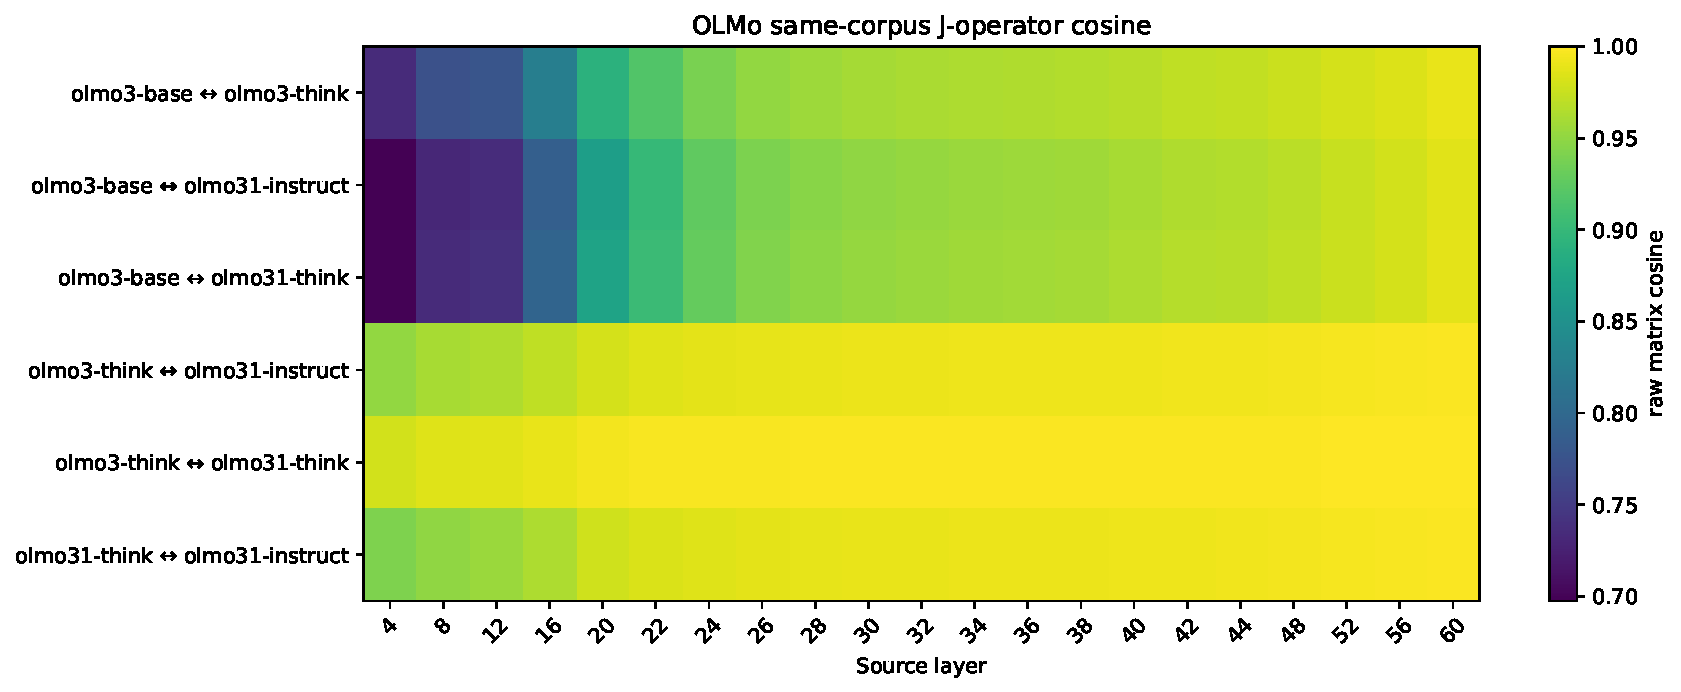
\includegraphics[width=0.98\textwidth]{olf01_operator_similarity_heatmap.pdf}
\caption{All-layer raw J-operator cosine for every checkpoint pair. Coarse
operator continuity is high overall but has localized early-layer movement.
Evidence: \eid{ol-geometry-figures-dev-v1}.}
\end{figure}

\subsection{Mapped token rows move at the first Think transition}

Base-to-3.0 raw-operator cosine has all-layer median 0.9614 and minimum 0.7343
at layer 4. Yet mapped token-row median cosine is only 0.6744, and the median
layer-level fifth percentile is 0.5950. By contrast, raw unembedding rows have
median cosine 0.9853. The discrepancy therefore lies primarily in the fitted J
mapping and its token geometry rather than gross output-weight movement.

\begin{figure}[H]
\centering
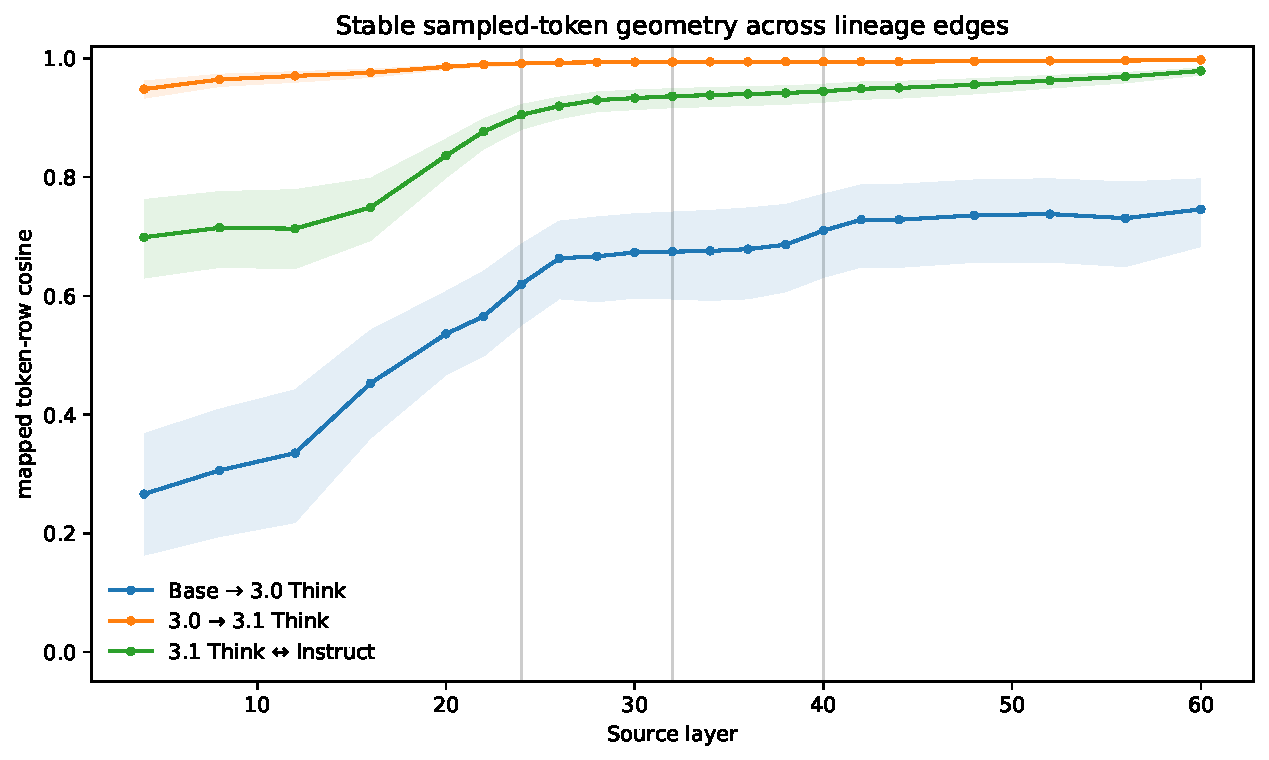
\includegraphics[width=0.88\textwidth]{olf02_token_row_similarity.pdf}
\caption{Mapped token-row cosine across source layers. Base-to-3.0 movement is
large, while 3.0-to-3.1 is nearly stationary. The Instruct series is a sibling
comparison, not a temporal continuation.}
\end{figure}

The frozen formation contrast is 0.32556 mapped movement for Base-to-3.0
versus 0.00604 for 3.0-to-3.1. The later Think edge has raw-operator/mapped-row
medians 0.99817/0.99396 and raw-unembedding median 0.999994. Thus the large
movement is localized to the first released Think transition, but the released
checkpoints do not identify which unobserved stage produced it.

\subsection{Selected spans reorganize despite stable capacity}

At layers 24/32/40, Base-to-3.0 median selected-ID Jaccard is 0.3333 at every
layer, with projector overlap 0.2657/0.3336/0.4549. The 3.0-to-3.1 selected-ID
Jaccard is 1.0 at all three layers and projector overlap is
0.9845/0.9895/0.9906.

\begin{figure}[H]
\centering
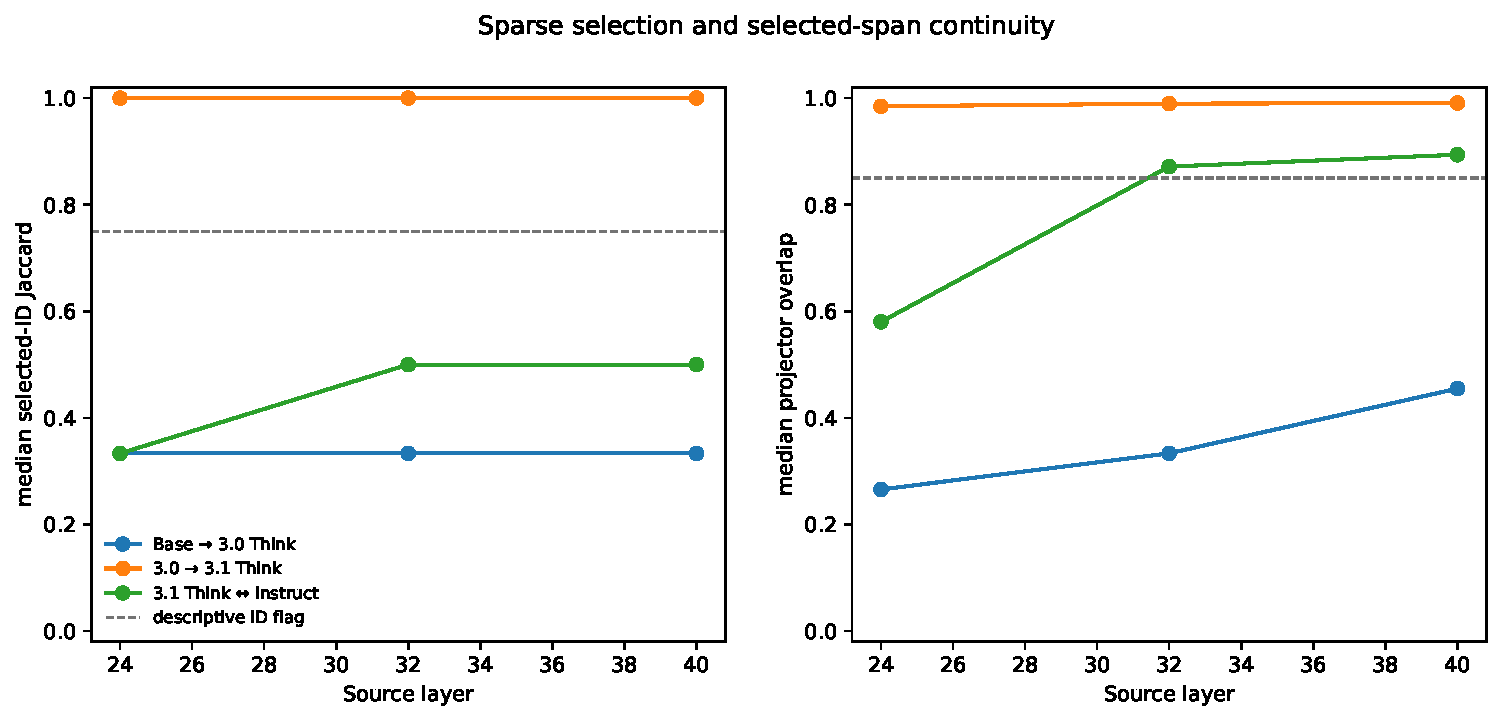
\includegraphics[width=0.95\textwidth]{olf03_selected_span_trajectory.pdf}
\caption{Selected-ID and selected-span continuity at the capacity layers.
Sparse occupancy can remain stable while the identities and span of selected
directions change substantially.}
\end{figure}

The complete router returns \texttt{dictionary-formation-pattern}: broad
operator continuity passes, mapped-token continuity fails, selection
divergence is true, the formation contrast is true, and the Instruct late-shift
flag is false \eid{ol-geometry-joint-dev-v1}.

\begin{statusbox}[title={Bounded sentence-2 interpretation}]
Across this architecture-matched lineage, the first released Think transition
is associated with strong J-mapped coordinate and selected-span reorganization
without material measured sparse-capacity growth. The result is not evidence
that the Think objective caused the dictionary, nor that a globally conserved
coordinate system is usable at finite intervention dose.
\end{statusbox}

\subsection{Capacity and known causal utilization are distinct axes}

\begin{figure}[H]
\centering
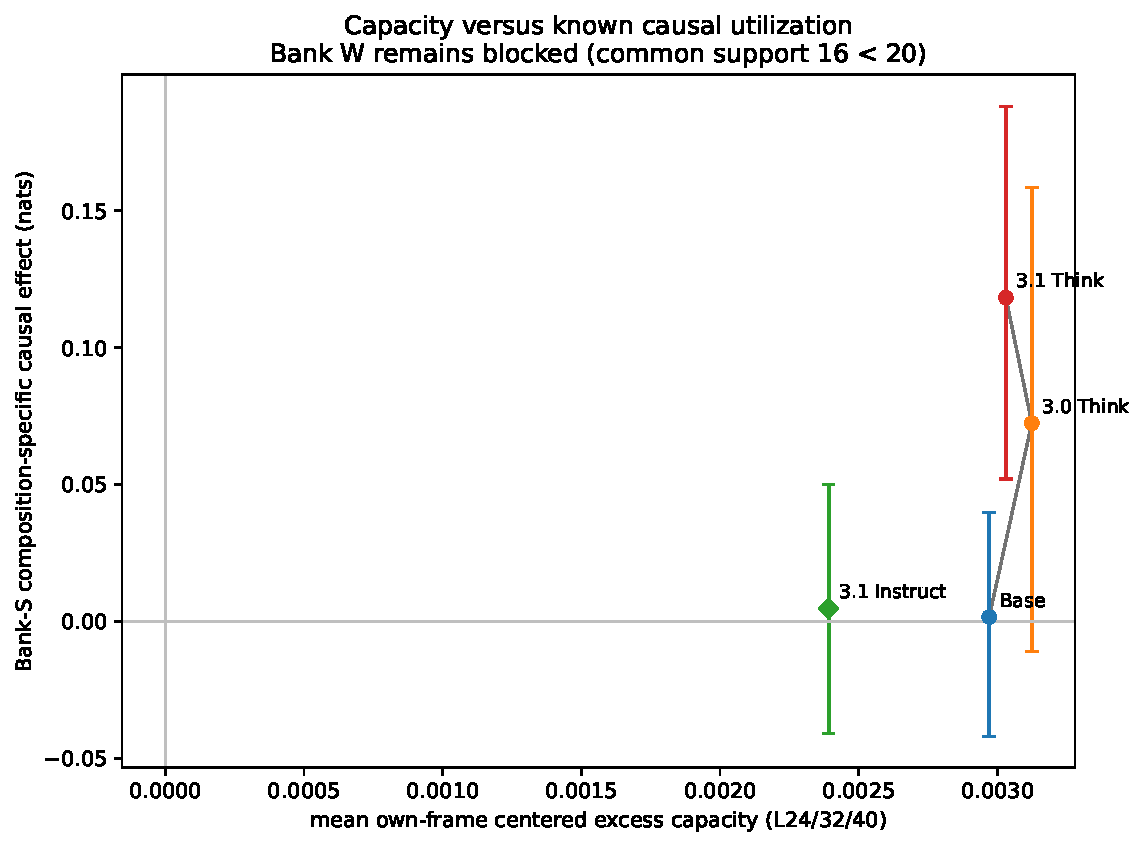
\includegraphics[width=0.72\textwidth]{olf04_capacity_causal_state_space.pdf}
\caption{Own-frame capacity against previously registered Bank-S causal
utilization. The causal axis is imported development evidence, not a Bank-W
or O4 result. The title records the 16/20 Bank-W gate.}
\end{figure}

The state-space view is useful precisely because it resists a scalar workspace
score: checkpoints with similar measured sparse capacity can differ in known
causal utilization. It is descriptive triangulation. The current OLMo track
did not rerun or open those Bank-S intervention outcomes.

\begin{figure}[H]
\centering
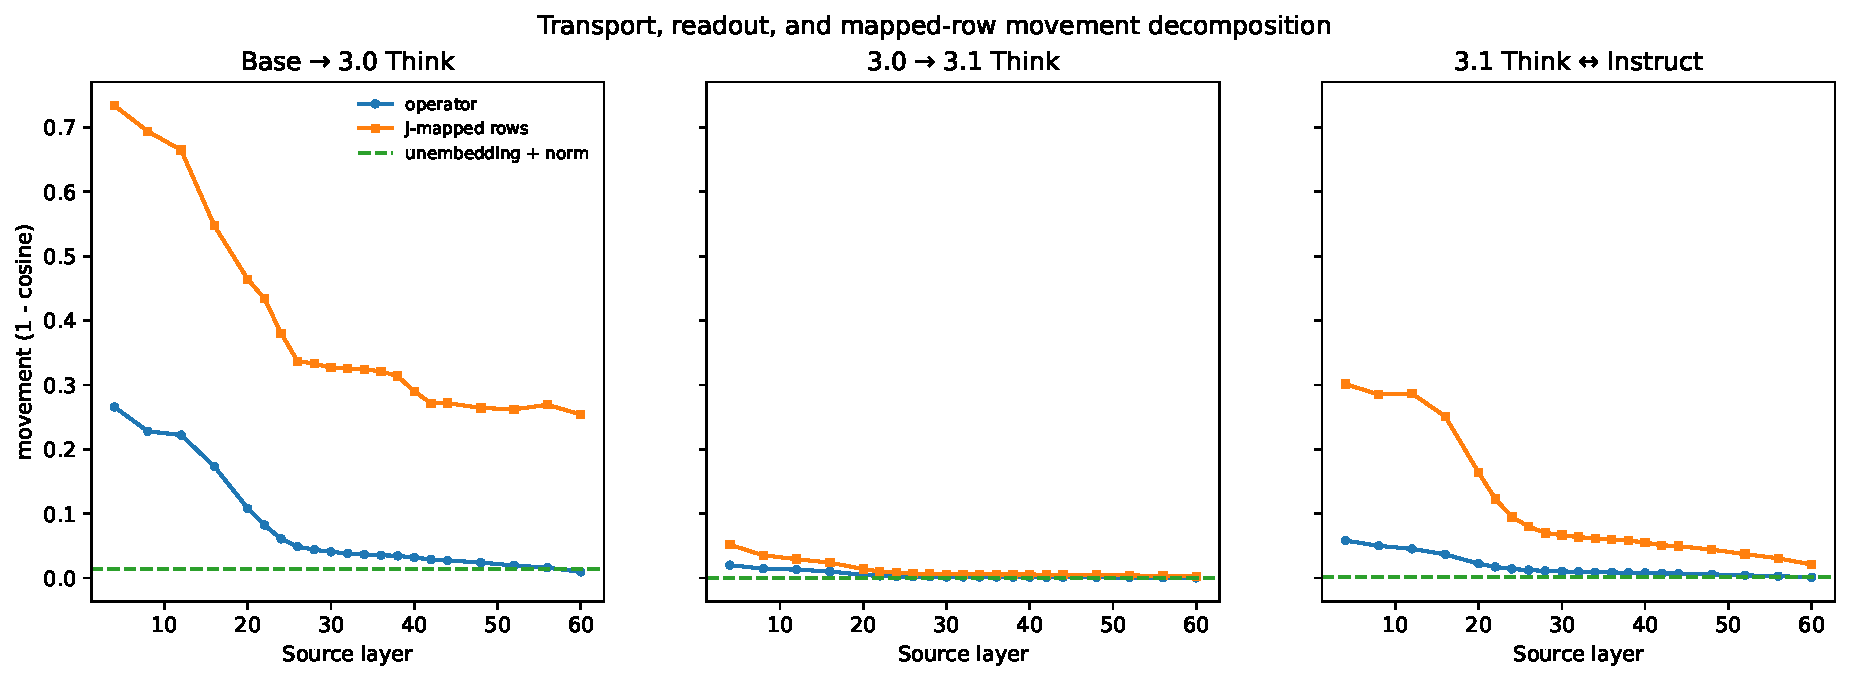
\includegraphics[width=0.98\textwidth]{olf05_readout_transport_decomposition.pdf}
\caption{Movement in the fitted operator, J-mapped rows, and raw
unembedding-plus-normalization readout. Structural similarity decomposes where
coordinates move; it does not itself establish finite-dose causal transport.}
\end{figure}

\section{Honest stopping decisions and Study-2 closure}

\subsection{O4 is gated out, not negative}

The four prospective Bank-W patterns were frozen before the gate: external-
state substitution, generic difficulty, capacity, and output-adjacent routing.
Because common support is 16/20, no load $\times$ derivation $\times$
redundancy intervention grid exists. Consequently, conclusion-skeleton
sentence 4 does not graduate.

The exact release wording is:

\begin{quote}
Existing Bank-S development evidence motivates an external-state-substitution
hypothesis on the tested Think checkpoints, but the planned fact-paired Bank-W
factorial was gated out at 16/20 common families; this release does not resolve
an externalization mechanism.
\end{quote}

\subsection{The official SFT/DPO wedge is capability-gated}

The official artifact inventory initially used byte-identical tokenizer files
and conservatively returned no eligible intermediate pair. A versioned semantic
audit showed that Think-SFT changes tokenizer serialization but preserves the
full 100,278-entry token-ID map, normalized 100,000 BPE merges, processing
components, and all 207 frozen encodings. Official 32B Think-SFT and Think-DPO
artifacts were therefore eligible \eid{ol-checkpoint-inventory-v2}. Study 2
then froze exact revisions, both registered lens frames, the complete
972-row Bank-F+S battery, seven intervention conditions, capability floors,
stage predictions, and route order before either model loaded
\eid{ol2-checkpoint-ancestry-v1} \eid{ol2-foundation-v1}.

Both checkpoints fail the prospective intervention-cohort gate. Exact
normalized-generation capability is 0.00617 at SFT and 0.00309 at DPO. Neither
checkpoint has a Bank-S fact capable on both direct and composed variants,
versus required floors of 72 facts and 20 families. Consequently, no
seven-condition intervention outcome exists under either frame
\eid{ol2-stage-wedge-think-sft-tier1-v1}
\eid{ol2-stage-wedge-think-dpo-tier1-v1}.

\begin{figure}[H]
\centering
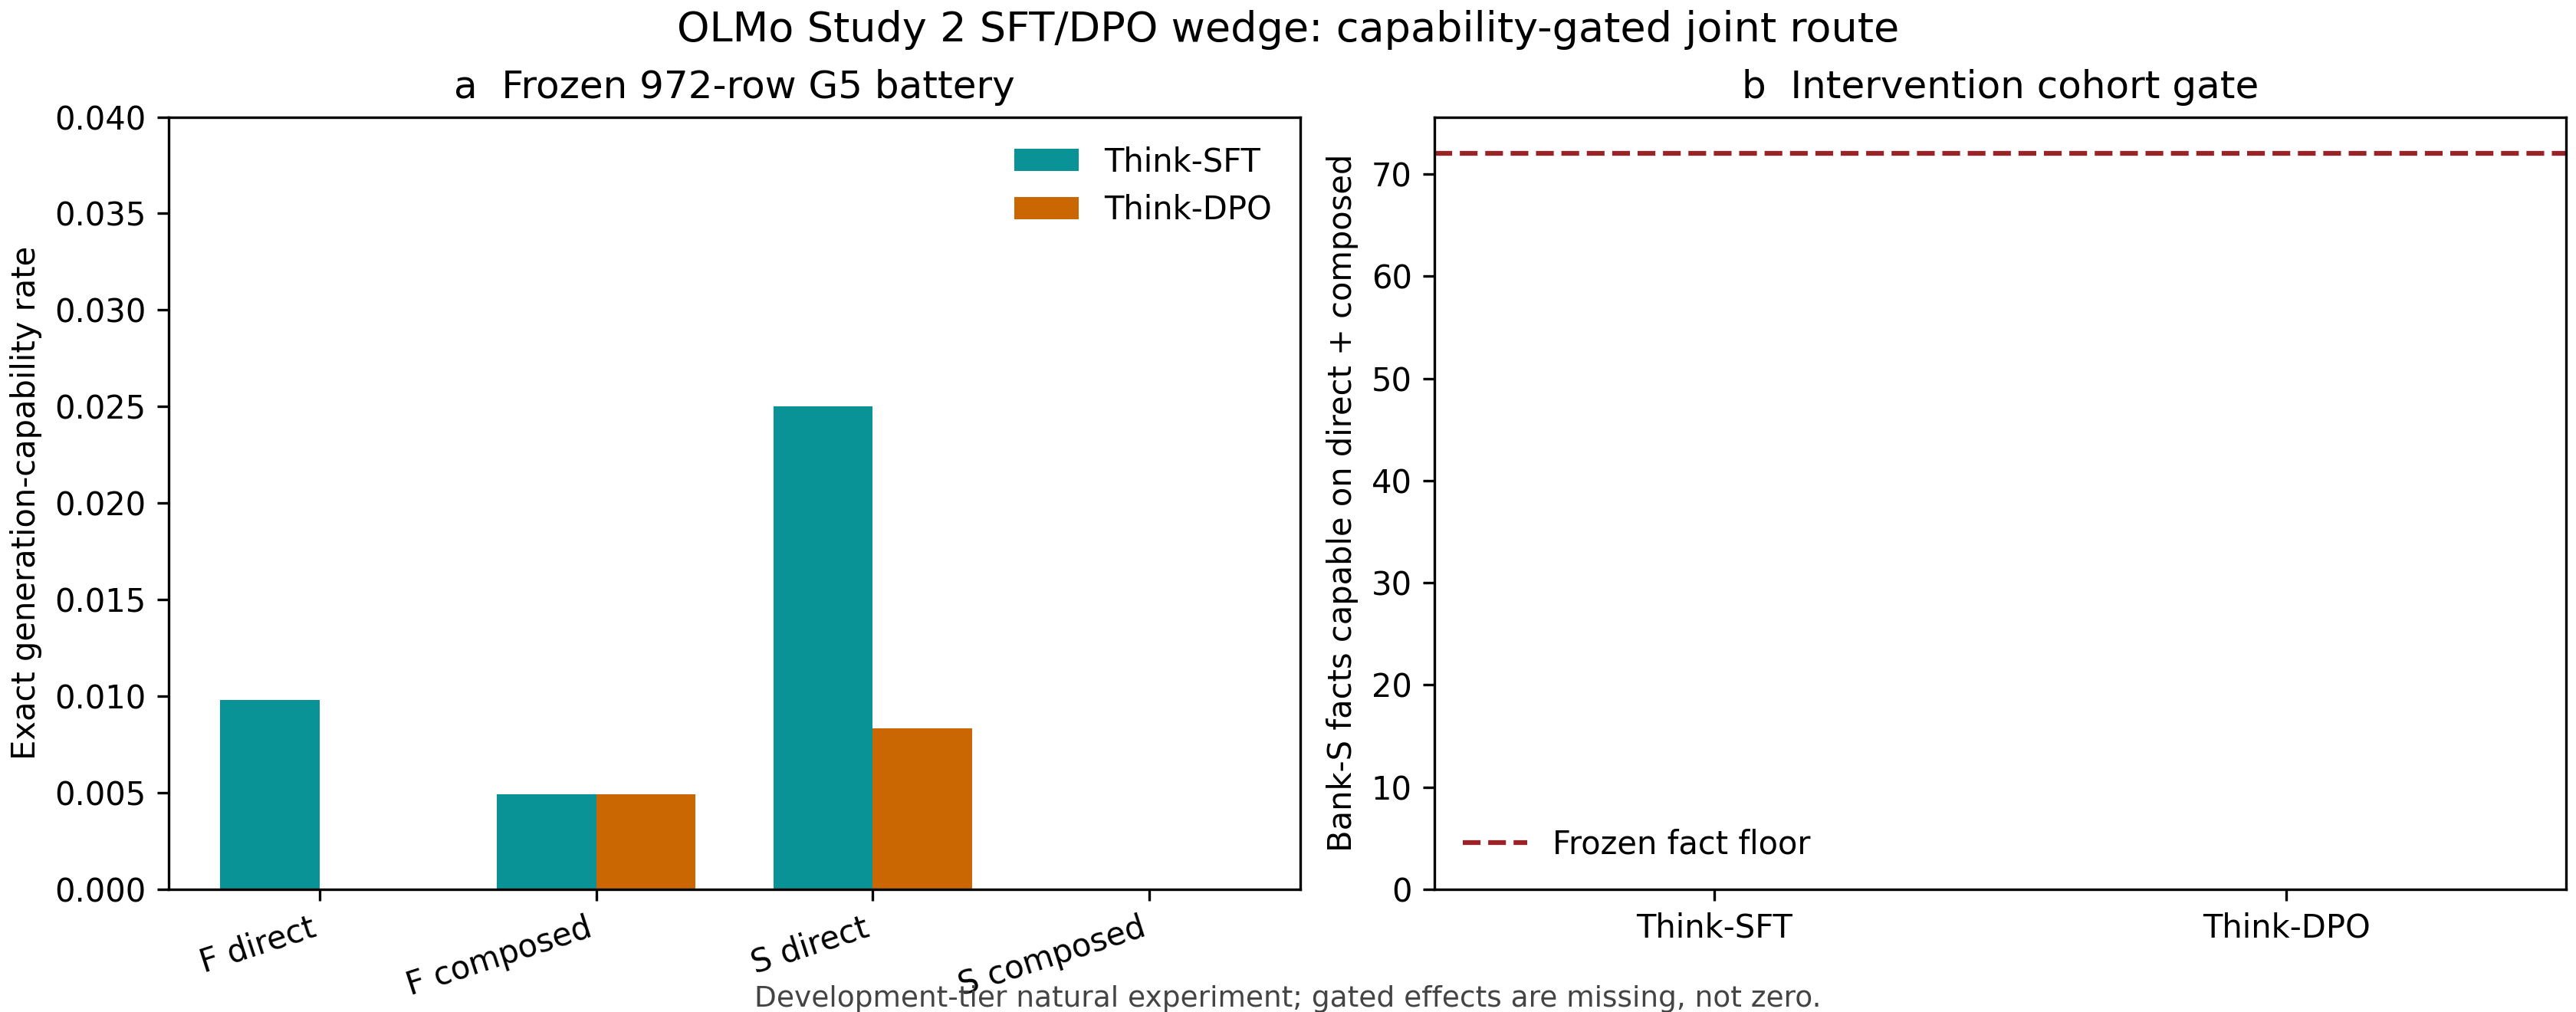
\includegraphics[width=0.90\textwidth]{ol2_stage_wedge_capability_route.png}
\caption{The frozen 972-row capability battery and Bank-S intervention-cohort
gate. Effects are missing, not zero. Evidence:
\eid{ol2-stage-wedge-joint-analysis-v1}.}
\end{figure}

The exact paired transition has 965 incapable-both items, two capable-both,
four lost-at-DPO, and one Bank-F bridge-supplied onset-at-DPO item. No Bank-S
direct+composed onset exists. The joint router selects
\texttt{null\_or\_unresolved}: the official SFT/DPO checkpoints do not
localize the first-release transition under the frozen assay. Later stages,
checkpoint spacing, capability limits, and measurement variation remain open.
The single Tier-2 lens-refit trigger is false.

\subsection{H6 fails in band and passes only a Think late anchor}

The exact registered Gemma calibration import licenses an OLMo-specific
dual-exact-JVP ceiling of 0.0787037; no pooled ceiling is used. Base and
OLMo-3.1 Think each contribute 336 rows: four prompts, layers 24/32/40/56,
three direction families, and seven frozen relative doses from 0.001 to 0.10.
All 672 backend comparisons pass the imported ceiling
\eid{ol2-gemma-backend-calibration-import-v1}
\eid{ol2-transport-execution-freeze-v1}.

\begin{table}[H]
\centering\small
\begin{tabular}{@{}lrrrrl@{}}
\toprule
\textbf{Checkpoint} & \textbf{Rows} & \textbf{Meas.} & \textbf{Decision} &
\textbf{Passing} & \textbf{Frozen route}\\
\midrule
Base & 336 & 34 & 13 & 9 & no licensed regime\\
OLMo-3.1 Think & 336 & 77 & 37 & 12 & late-anchor-only\\
\bottomrule
\end{tabular}
\caption{H6 row disposition. Passing rows alone do not define a layer-dose
pass; the prospective passage floor is 0.90 within each 12-row cell.}
\end{table}

\begin{figure}[H]
\centering
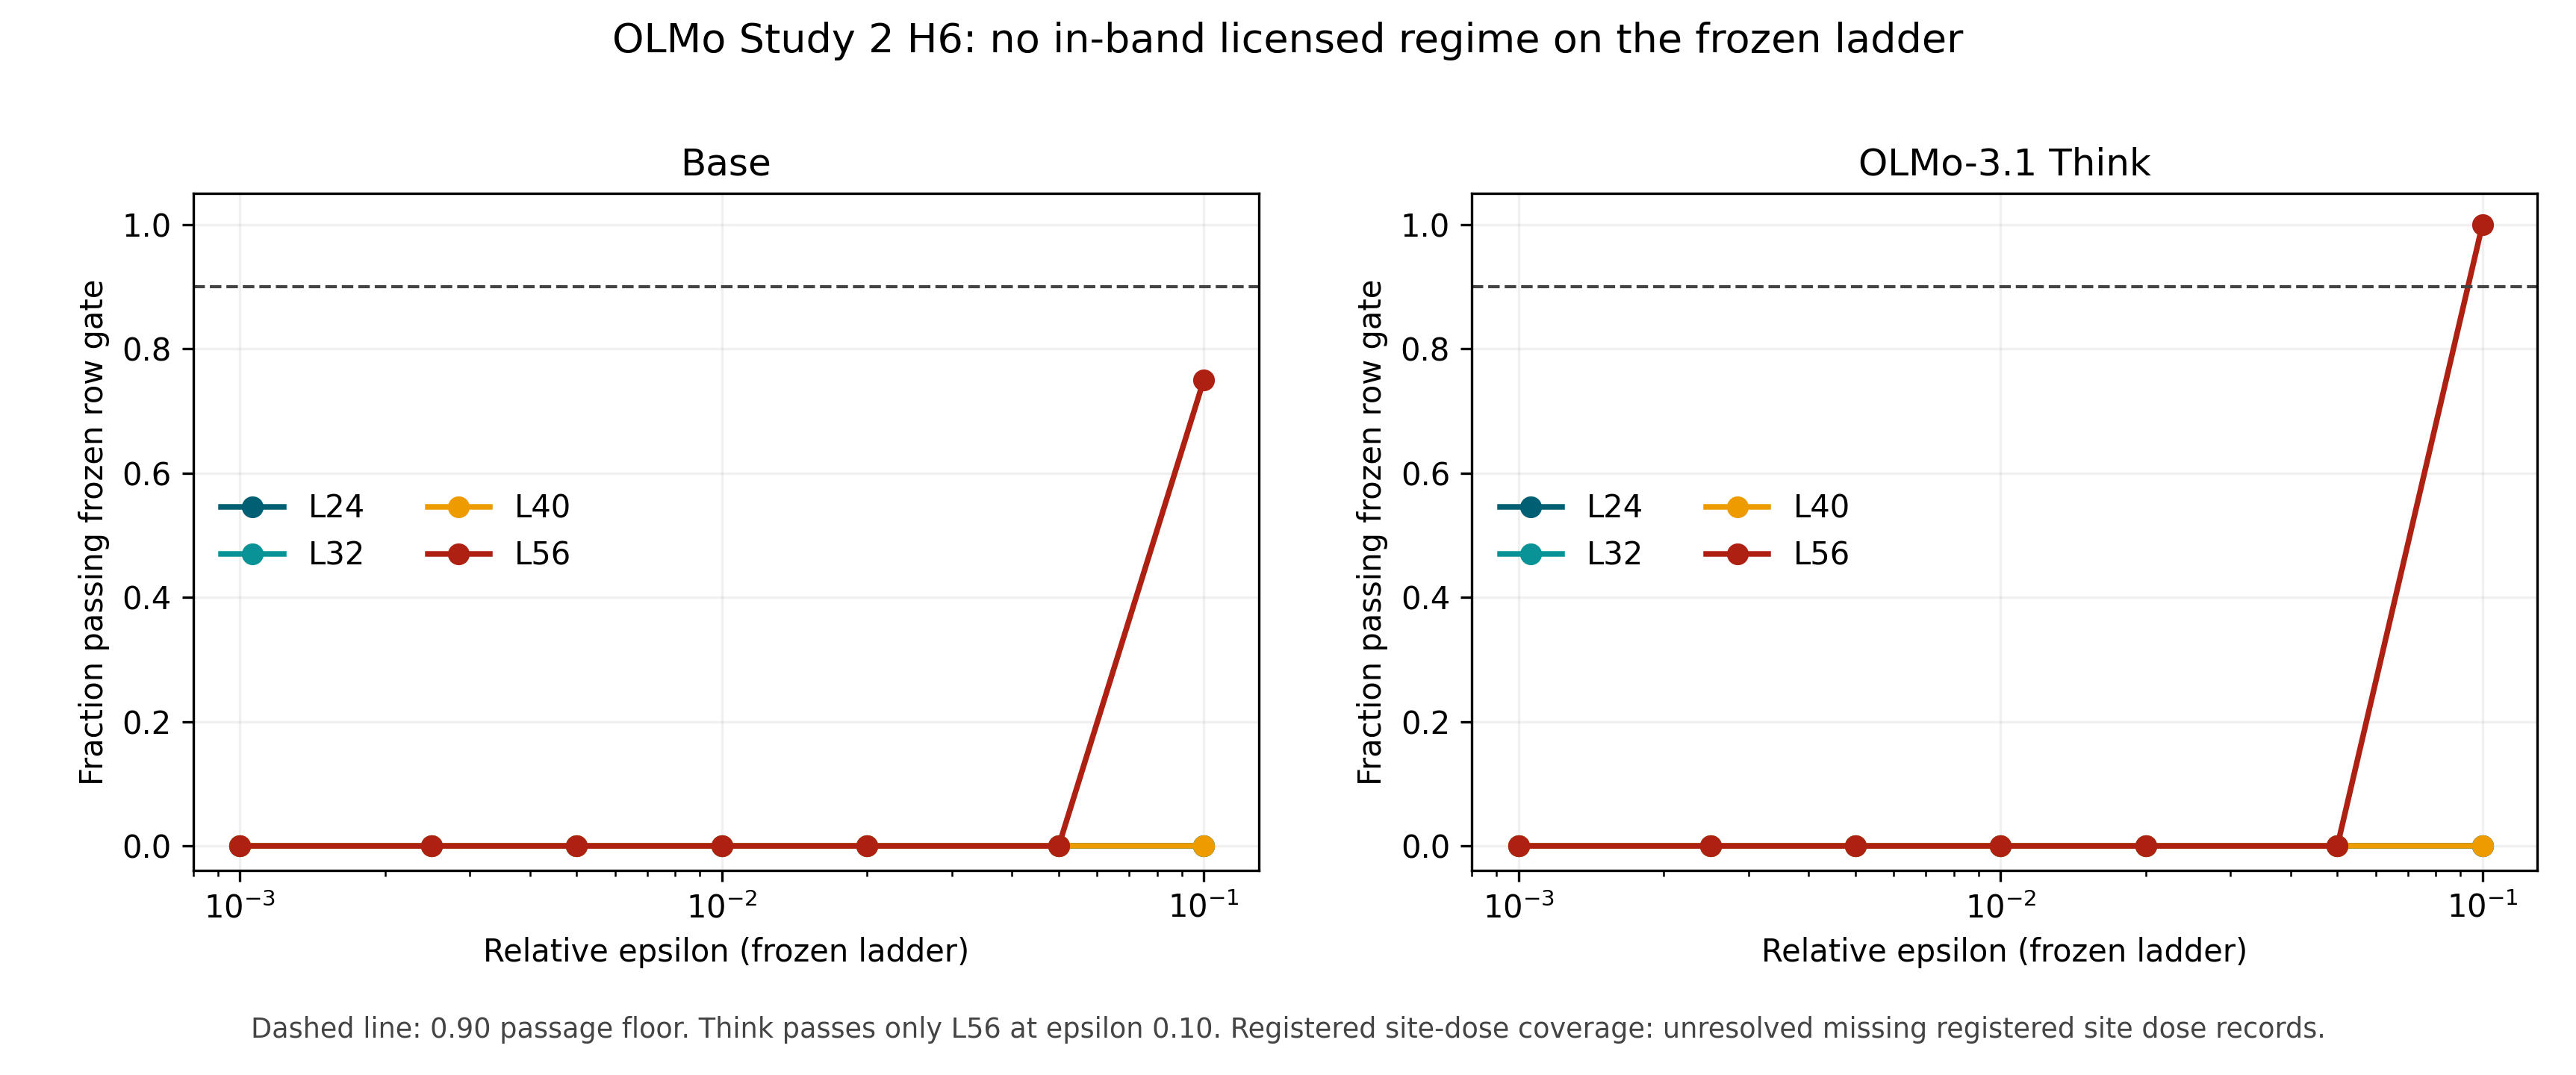
\includegraphics[width=\textwidth]{ol2_transport_validation_joint_paper.png}
\caption{Frozen passage fractions by checkpoint, layer, and dose. No
L24/L32/L40 cell passes. Think passes only L56 at $\epsilon=0.10$; Base reaches
9/12 there and remains below the 0.90 floor. Evidence:
\eid{ol2-transport-validation-joint-v1}
\eid{ol2-transport-validation-figure-v1}.}
\end{figure}

The joint route is
\texttt{h6\_fail\_in\_band\_with\_checkpoint\_specific\_late\_anchor}.
This narrows transport wording and does not invalidate the registered paired
ablation effects. A registered-source audit finds no exact OLMo site table
containing item/layer/position, total removed-energy fraction, and the frozen
residual-norm conversion together. Per-item means/maxima and per-position
protected-subspace energy are not substitutes. Causal-dose coverage therefore
remains unavailable, not zero.

\subsection{O5 is not identifiable from structural proxies}

The registry has capacity and structural geometry, but no causal rows that
independently cross activation model, transport lens, and output readout. H6
now supplies per-checkpoint average/prompt transport on the frozen ladder, but
it does not supply per-dictionary crossed transport, protected-span geometry under
each readout, delivered rank/energy checks, a non-J logit-lens baseline, and a
fixed common crossed-row order. The registered decision is
\texttt{defer-no-identifiable-crossed-intervention-estimand} and
\texttt{not-executed-no-proxy-substitution}
\eid{ol-o5-feasibility-decision-v1}. No factor estimate or null is reported.

\section{Independent reconstruction}

Every headline result was reconstructed outside the production aggregation
path from registered sufficient statistics. The methods event checks:

\begin{itemize}
  \item 768 Bank-W rows, all candidate-score identities, load/family accuracy,
    deterministic family bootstraps, and the 16/20 intersection;
  \item 48 capacity curve summaries, 96 prompt-bootstrap intervals, 144 joint
    arrays, and all 72 joint-table rows;
  \item 84 geometry aggregates, the complete router, six readout rows, and all
    protected null boundaries;
  \item five regenerated PNGs byte-for-byte and five valid regenerated PDFs;
  \item every metadata file and all fourteen exact OLMo-3.1 Think weight
    shards; and
  \item one frozen Bank-W row under the original eight-candidate batch: all
    eight log probabilities, predicted alias, prompt/token manifest, and
    $-0.25$ margin reproduce with maximum drift exactly zero.
\end{itemize}

The result is \eid{ol-independent-reconstruction-v1}. Its JSON SHA-256 begins
\texttt{e159f01d}; the payload hash begins \texttt{ee94e446}. This is
computational reconstruction, not a new confirmatory cohort and not a tier
upgrade.

Two rejected pre-publication attempts are part of the audit trail. The first
omitted the original producer's \texttt{no\_grad} context and exhausted VRAM
after all weight hashes passed. A one-candidate diagnostic fit but changed BF16
batch numerics (maximum drift 0.20499 nats; margin $-0.125$ instead of
$-0.25$), so it was rejected without weakening tolerance. Restoring
\texttt{no\_grad} and the frozen batch reproduced every value exactly. Neither
failed attempt created a registry event or durable result.

\section{Claim ledger and Phase 5 router}

\begin{table}[H]
\centering\small
\begin{tabularx}{\textwidth}{@{}
  >{\raggedright\arraybackslash}p{0.12\textwidth}
  >{\raggedright\arraybackslash}p{0.20\textwidth}
  >{\raggedright\arraybackslash}X@{}}
\toprule
\textbf{Target} & \textbf{Disposition} & \textbf{Licensed wording}\\
\midrule
Sentence 2 & narrowed; release-resolved & architecture-matched
association between the first Think transition and J-mapped coordinate/
selection reorganization without material measured capacity growth; the
official SFT/DPO wedge does not stage-localize it, and H6 does not license an
L24/L32/L40 finite-dose regime\\
Sentence 4 & explicitly pending & Bank-S motivates externalization, but the
Bank-W factorial was gated out at 16/20 and resolves no mechanism\\
H5 & null or unresolved & both official stage cohorts are capability-gated;
intervention effects are missing and no SFT/DPO boundary is localized\\
H6 & fail in band; Think late-only & neither checkpoint passes L24/L32/L40;
Think alone passes L56 at $\epsilon=0.10$; registered dose coverage is
unavailable rather than zero\\
O5 & not identifiable & no activation/lens/readout factor estimate or null;
structural proxies are not substituted\\
\bottomrule
\end{tabularx}
\caption{Paper-facing claim resolution. The sentence-level source of truth is
\nolinkurl{OLMO_LINEAGE_CLAIMS_TABLE_V2.md}.}
\end{table}

The next integrated phase receives three bounded entries:

\begin{enumerate}
  \item a newly prospective, capability-compatible stage assay if stage
    localization remains important; the gated official wedge is not repaired;
  \item exact per-position total-dose and residual-norm logging in any future
    causal producer before intervention-relevant H6 coverage is claimed; and
  \item only then, a Bank-S-first Base/3.1-Think/3.1-Instruct pilot crossing Base versus
    recipient-own transport and readout, expanded only after protected-span,
    delivered-rank, and delivered-energy checks pass.
\end{enumerate}

Bank W remains closed under version 1. Any redesigned service population is a
new prospective study, not a subset repair.

\section{Limitations}

\begin{enumerate}
  \item \textbf{Natural experiment.} The lineage localizes checkpoint
    associations but does not randomize training data, objective, or stage.
  \item \textbf{Measured capacity.} Stability applies to the frozen corpus,
    layers, dictionary, persistence rule, random controls, and equivalence
    margin. It is not a theorem about all internal capacity.
  \item \textbf{Transport.} H6 is measured on four prompts and three frozen
    directions. It finds no in-band passing cell on the tested ladder, but
    exact intervention-dose coverage remains unavailable because the
    registered archive lacks the required site stream.
  \item \textbf{Stage wedge.} Both official intermediate checkpoints fail the
    prospective capability cohort. Missing intervention effects cannot be
    treated as zero or as evidence for either training boundary.
  \item \textbf{Externalization.} O4 is absent because the service population
    failed prospectively. Existing Bank-S evidence cannot choose the Bank-W
    mechanism account.
  \item \textbf{Missing margins.} Exact kth/k+1 candidate-correlation gaps,
    protected-span overlap under crossed readouts, and core/fringe causal dose
    remain null.
  \item \textbf{Sibling endpoint.} Instruct is not a temporal successor and
    cannot be used to infer reversal along the Think path.
  \item \textbf{Tier.} Reconstruction improves reliability, not evidentiary
    tier. No OLMo-native result is confirmatory or replication evidence.
\end{enumerate}

\begin{warningbox}[title={Prohibited conclusions}]
This release does not license ``Think training creates a global workspace,''
``the reasoning objective is the causal variable,'' ``reasoning post-training
installs external-state substitution,'' ``the dictionaries are identical,''
``the stage effect is zero,'' ``the causal-dose coverage is zero,'' or
``Instruct lacks a verbalizable channel.''
\end{warningbox}

\section{Conclusion}

The OLMo lineage closes the most important capacity hole in the earlier
trajectory. Base does not show a materially smaller value under the symmetric
sparse-capacity estimator, yet the first released Think transition reorganizes
J-mapped token rows and selected spans far more than the later Think transition.
This combination favors a careful description: capacity is stable under the
measured assay while coordinate/selection organization is not.

The study is equally informative where it stops. A 16/20 prospective service
failure prevents the decisive Bank-W externalization grid; the official
SFT/DPO wedge opens no intervention cohort; and the H6 assay band has no
licensed passing regime on the frozen ladder. OLMo-3.1 Think's isolated L56
pass does not rescue in-band wording. Exact intervention-dose coverage also
remains unavailable rather than zero. These boundaries favor new prospective
capability and site-dose instrumentation over an overextended mechanism claim.

\appendix
\section{Evidence and artifact index}

\begin{tabularx}{\textwidth}{@{}p{0.34\textwidth}p{0.13\textwidth}X@{}}
\toprule
\textbf{Evidence} & \textbf{Tier} & \textbf{Role}\\
\midrule
\nolinkurl{ol-foundation-v1} & methods & isolation, imports, environment,
preregistration\\
\nolinkurl{ol-bank-w-capability-joint-dev-v1} & development & exact 16/20
service decision\\
\nolinkurl{ol-phase4-early-import-bundle-v1} & methods & early hash-pinned
Phase 4 capability handoff\\
\nolinkurl{ol-lens-provenance-audit-v1} & methods & exact same-recipe/corpus
classification\\
\nolinkurl{ol-capacity-joint-dev-v1} & development & paired symmetric capacity
router\\
\nolinkurl{ol-geometry-joint-dev-v1} & development & all-layer and selected-
span geometry router\\
\nolinkurl{ol-geometry-figures-dev-v1} & development & five registered figure
pairs\\
\nolinkurl{ol-checkpoint-inventory-v2} & methods & official SFT/DPO eligibility
and Study-2 entry\\
\nolinkurl{ol2-stage-wedge-joint-analysis-v1} & development & paired official
SFT/DPO capability route; effects missing\\
\nolinkurl{ol2-gemma-backend-calibration-import-v1} & methods & exact
OLMo-specific backend ceiling import\\
\nolinkurl{ol2-transport-validation-joint-v1} & methods & 672-row H6 joint
router and registered-dose archive audit\\
\nolinkurl{ol2-transport-validation-figure-v1} & methods & paper-facing H6
figure derivative\\
\nolinkurl{ol-o5-feasibility-decision-v1} & methods & no-substitution
identifiability decision\\
\nolinkurl{ol-independent-reconstruction-v1} & methods & independent tables,
figures, hashes, and model sentinel\\
\bottomrule
\end{tabularx}

\section{Key immutable hashes}

\begin{itemize}
  \item Scientific boundary:
    \texttt{3b041735d8b842de46a9c0a474fccd0c44e0841a}.
  \item Early handoff JSON:
    \texttt{debb29ef67ffa8741a4971ec2b0b21340bd5b48dc5729ac12f74f78839bf4f2b}.
  \item Capacity joint JSON: \texttt{cb35a22a...d1492}.
  \item Capacity table: \texttt{b3ad02e9...e247e}; paired bootstrap:
    \texttt{c13cebed...10fa}.
  \item Geometry joint JSON: \texttt{c09d8e73...d0f4c}.
  \item Geometry layer table: \texttt{8692836d...9097}; selection table:
    \texttt{c2826b14...73bd}.
  \item Geometry readout table: \texttt{93fd2108...0bd9}.
  \item Inventory v2 JSON: \texttt{e5931c3f...ad9a}.
  \item O5 decision JSON: \texttt{d31d23e4...74499}.
  \item Reconstruction JSON: \texttt{e159f01d...20542}; payload:
    \texttt{ee94e446...619f}.
  \item Stage-wedge joint JSON: \texttt{44882a8d...9357}.
  \item H6 Base result: \texttt{401737b9...e69d0}; Think result:
    \texttt{747483bf...f4e73}.
  \item H6 joint JSON: \texttt{e563dfbe...8a33}.
  \item H6 paper PNG/PDF: \texttt{03564b35...a7b1} and
    \texttt{b2745d9e...d610}.
\end{itemize}

\section{Operational reproducibility}

The append-only Git registry is authoritative for event order; the isolated
Drive root is authoritative for heavy outputs. Before the Study-2 release
event, 35 live events and 142 live outputs verify. The stable Study-2 handoff is
\nolinkurl{reports/INPROGRESS_OLMO_LINEAGE_2.md}; the versioned scientific
snapshot is \nolinkurl{reports/OLMO_LINEAGE_STATE_OF_RECORD_V2.md}; and the
sentence-level license is
\nolinkurl{reports/OLMO_LINEAGE_CLAIMS_TABLE_V2.md}.

\end{document}
